\documentclass[brazil]{article}
\usepackage{graphicx}
\usepackage[T1]{fontenc}
\usepackage[utf8]{inputenc}
\usepackage{babel}
\usepackage{url}


\begin{document}

\title{Carta de Motivação para Financiamento via Pró-Int de Participação em Evento como Palestrante}


\maketitle

\begin{flushleft}
À Comissão de Graduação do IME/USP,
\end{flushleft}

%\begin{abstract}
%\end{abstract}


Sou aluno do $7^{o}$ semestre do BCC e estou no segundo ano de iniciação científica no projeto Apoio BCC (\url{http://bcc.ime.usp.br}), coordenado pelo Professor do DCC, José Coelho de Pina e financiado pela Pró-Reitoria de Graduação no programa Ensinar com Pesquisa. Dentre um dos resultados do projeto está a confecção do artigo em anexo orientado pelo coordenador pedagógico do IME, Giuliano Olguin, que visa analisar o enfoque matemático de onze cursos de Ciência da Computação do Brasil e compará-los com dois currículos de referência. 

Conforme e-mail anexado a esta carta, o resumo foi aprovado no IEEE Frontiers In Education Conference 2013 (\url{http://fie2013.org}). O envio da versão completa do artigo está prevista para 8 de abril, e a notificação de aceite para o dia 8 de maio. O evento se dará dos dias 23 a 26 de outubro em Oklahoma City, no estado de Oklahoma, EUA.

Desta forma, gostaria de requisitar o financiamento da viagem de apresentação deste artigo através de verba do programa Pró-Int. Uma descrição do evento e um orçamento dos gastos previstos encontram-se anexos. Permaneço à disposição para quaisquer dúvidas.

\vfill

\begin{flushright}
\line(1,0){200}\\
Pedro Paulo Vezzá Campos\\
Projeto Apoio BCC\\
\url{pedrovc@ime.usp.br}\\
(11) 97132-1145
\end{flushright}

\newpage 

\section{Sobre o IEEE Frontiers In Education Conference 2013 (FIE2013)}
O $43^o$ congresso anual Frontiers in Education (FIE) é um evento internacional de grande importância, recebendo classificação QUALIS área Computação B1 e possuindo índice-H 24. Suas principais temáticas são sobre inovações educacionais e pesquisa em engenharia e computação. O FIE2013 continua uma longa tradição de disseminar resultados nestas áreas. Seus organizadores afirmam ser um um fórum ideal para compartilhar ideias, aprender sobre desenvolvimentos em Ciência da Computação, engenharia e educação tecnológica e interagir com colegas nestas áreas.

Os patrocinadores do evento são: Institute of Electrical and Electronics Engineers (IEEE), IEEE Education Society, IEEE Computer Society, American Society for Engineering Education (ASEE) e Educational Research Methods (ERM) Division.

Maiores informações podem ser obtidas pelo site do evento: \url{http://fie2013.org}.

\section{Orçamento}
Valores em dólares foram convertidos considerando o câmbio de U\$1,00 = R\$1,95.

\subsection{Inscrição no Evento}
Para estudantes em tempo integral, o FIE2013 estipula uma taxa de inscrição de R\$682,50.

\subsection{Passagem Aérea}
Os valores informados abaixo foram coletados do site \url{decolar.com} no dia 12 de março. Para controlar o \emph{jet lag} de uma viagem de mais de 15 horas foram orçadas passagens com ida na noite do dia 21 de outubro, com chegada na tarde do dia 22. A volta seria no próprio dia 26.

\subsection{Hospedagem e traslado}
Verificando no \url{decolar.com} é possível encontrar hotéis na faixa de R\$86 por noite. O traslado aeroporto -- hotel custaria em torno de R\$29,25 para estes e o traslado hotel -- centro de convenções em torno de R\$37,05, de acordo com o \url{taxifarefinder.com}. O valor total incluindo 4 noites, traslado aeroporto -- hotel -- aeroporto e 4 traslados hotel -- centro de convenções -- hotel estaria na faixa de R\$698,90. Os valores dos hotéis recomendados pela organização do evento foram maiores que os cotados.

\subsection{Alimentação}
A inscrição no FIE2013 garante dois almoços, um na quinta 24 e outro na sexta 25. Assim, seriam necessários um jantar no dia 22, almoço e jantar no dia 23, apenas jantar nos dias 24 e 25 e almoço no dia 26, um total de 6 refeições. Cada uma foi estimada em R\$19,50.

\subsection{Totais}
\begin{description}
	\item[Inscrição] R\$682,50
	\item[Passagem Aérea] R\$2595,00
	\item[Hospedagem e traslado] R\$698,90
	\item[Alimentação] R\$117,00
	\item[Total] R\$4093,40
\end{description}

%\usepackage{graphics} is needed for \includegraphics
\begin{figure}[htp]
\begin{center}
  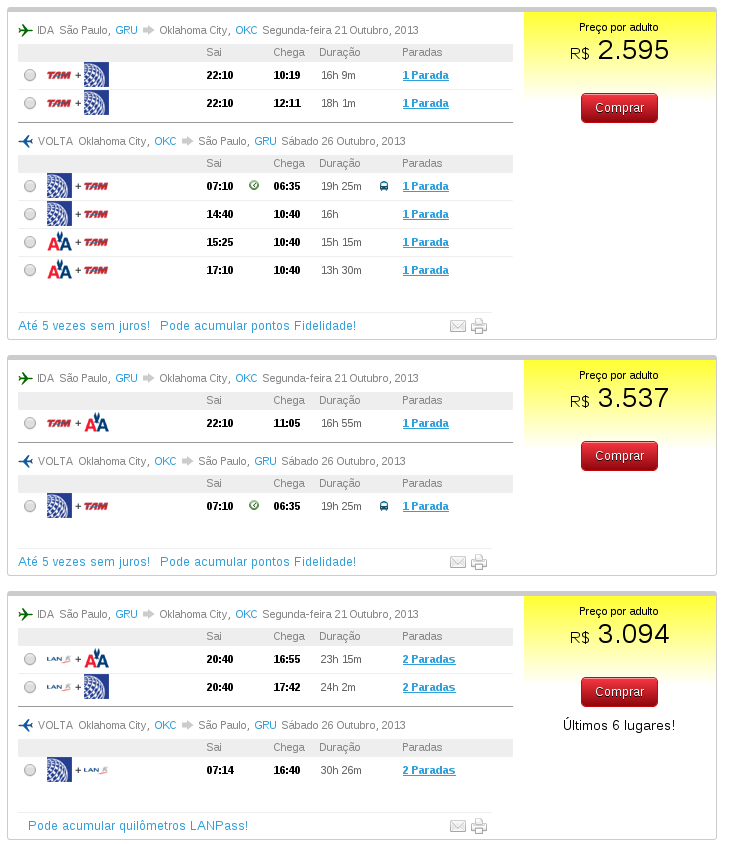
\includegraphics[width=\linewidth]{21-26.png}
  \caption[Opções de passagens aéreas com partida no dia 21 e retorno dia 26]{Opções de passagens aéreas com partida no dia 21 e retorno dia 26}
\end{center}
\end{figure}

%\usepackage{graphics} is needed for \includegraphics
\begin{figure}[htp]
\begin{center}
  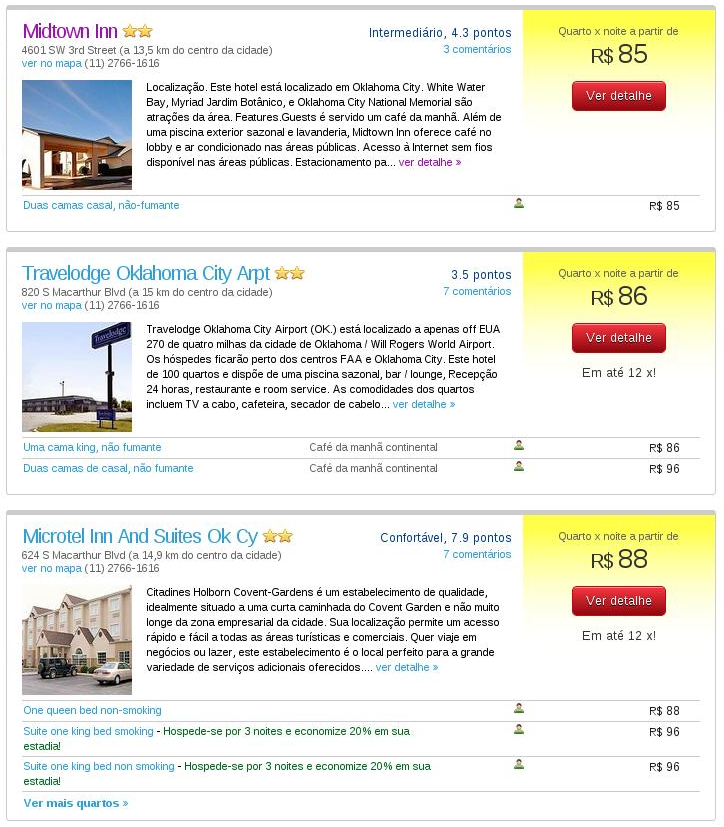
\includegraphics[width=\linewidth]{hoteis.png}
  \caption[Opções de hotéis]{Opções de hotéis}
\end{center}
\end{figure}


\end{document}

